\begin{figure}
	\centering
	\resizebox{\textwidth}{!}{
		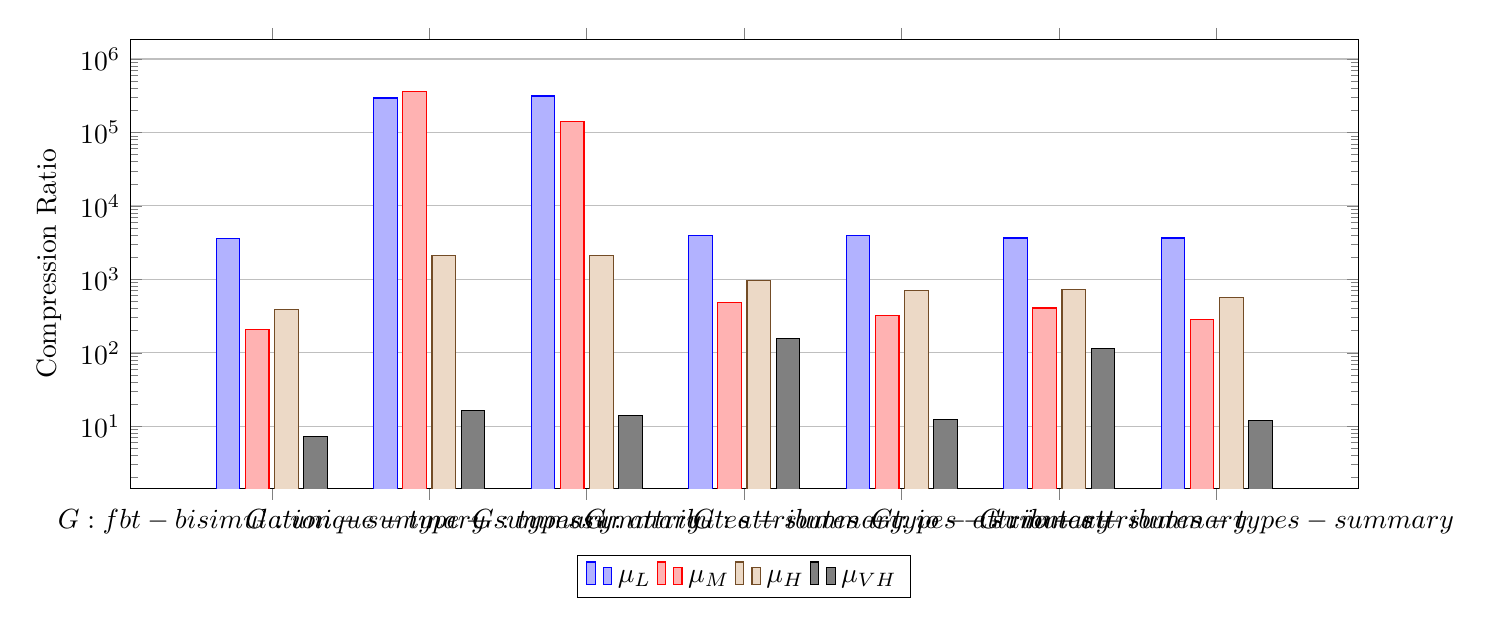
\begin{tikzpicture}
		\begin{axis}[
			ybar,
			symbolic x coords={$G:\glssymbol{fbt-bisimulation-summary}$,$G:\glssymbol{unique-type-summary}$,$G:\glssymbol{typessummary}$,$G:\glssymbol{attributes-summary}$,$G:\glssymbol{attributes-types-summary}$,$G:\glssymbol{io-attributes-summary}$,$G:\glssymbol{io-attributes-types-summary}$},
			enlargelimits=0.15,
			ylabel={Compression Ratio},
			x=2cm,
			bar width=0.3cm,
			xtick=data,
			ymode = log,
			ymajorgrids = true,
			legend style={at={(0.5,-0.15)},
			anchor=north,legend columns=-1},
		]
		\addplot coordinates {
			($G:\glssymbol{fbt-bisimulation-summary}$, 3589.49)
			($G:\glssymbol{unique-type-summary}$, 294067.89)
			($G:\glssymbol{typessummary}$, 313917.10)
			($G:\glssymbol{attributes-summary}$, 3999.70)
			($G:\glssymbol{attributes-types-summary}$, 3999.69)
			($G:\glssymbol{io-attributes-summary}$, 3654.78)
			($G:\glssymbol{io-attributes-types-summary}$, 3654.77)
		};

		\addplot coordinates {
			($G:\glssymbol{fbt-bisimulation-summary}$, 205.80)
			($G:\glssymbol{unique-type-summary}$, 361299.27)
			($G:\glssymbol{typessummary}$, 141978.05)
			($G:\glssymbol{attributes-summary}$, 490.00)
			($G:\glssymbol{attributes-types-summary}$, 326.39)
			($G:\glssymbol{io-attributes-summary}$, 407.85)
			($G:\glssymbol{io-attributes-types-summary}$, 283.95)
		};

		\addplot coordinates {
			($G:\glssymbol{fbt-bisimulation-summary}$, 386.79)
			($G:\glssymbol{unique-type-summary}$, 2103.26)
			($G:\glssymbol{typessummary}$, 2128.70)
			($G:\glssymbol{attributes-summary}$, 959.60)
			($G:\glssymbol{attributes-types-summary}$, 710.87)
			($G:\glssymbol{io-attributes-summary}$, 717.87)
			($G:\glssymbol{io-attributes-types-summary}$, 572.57)
		};

		\addplot coordinates {
			($G:\glssymbol{fbt-bisimulation-summary}$, 7.29)
			($G:\glssymbol{unique-type-summary}$, 16.21)
			($G:\glssymbol{typessummary}$, 14.08)
			($G:\glssymbol{attributes-summary}$, 154.86)
			($G:\glssymbol{attributes-types-summary}$, 12.34)
			($G:\glssymbol{io-attributes-summary}$, 113.75)
			($G:\glssymbol{io-attributes-types-summary}$, 12.04)
		};
		\legend{$\mu_L$,$\mu_M$,$\mu_H$,$\mu_{VH}$}
		\end{axis}
		\end{tikzpicture}
	}
	\caption{Compression ratio $G:\mathcal{S}$ of graph summaries. The ratio axis is reported in logarithmic scale.}
	\label{fig:vol-ration-bar}
\end{figure}

%\begin{figure}
%	\centering
%	\resizebox{\textwidth}{!}{
%		\begin{tikzpicture}
%		\begin{axis}[
%		ybar,
%		symbolic x coords={\glssymbol{unique-type-summary},\glssymbol{typessummary},\glssymbol{attributes-summary},\glssymbol{attributes-types-summary},\glssymbol{io-attributes-summary},\glssymbol{io-attributes-types-summary}},
%		enlargelimits=0.15,
%		ylabel={Compression Ratio},
%		x=2cm,
%		bar width=0.3cm,
%		xtick=data,
%		legend style={at={(0.5,-0.15)},
%			anchor=north,legend columns=-1},
%		]
%		\addplot coordinates {
%			(\glssymbol{unique-type-summary},1.89)
%			(\glssymbol{typessummary},1.77)
%			(\glssymbol{attributes-summary},81.73)
%			(\glssymbol{attributes-types-summary},81.74)
%			(\glssymbol{io-attributes-summary},89.57)
%			(\glssymbol{io-attributes-types-summary},89.57)
%		};
%
%		\addplot coordinates {
%			(\glssymbol{unique-type-summary},0.23)
%			(\glssymbol{typessummary},0.22)
%			(\glssymbol{attributes-summary},42.51)
%			(\glssymbol{attributes-types-summary},53.37)
%			(\glssymbol{io-attributes-summary},51.45)
%			(\glssymbol{io-attributes-types-summary},62.68)
%		};
%
%		\addplot coordinates {
%			(\glssymbol{unique-type-summary}, 17.81)
%			(\glssymbol{typessummary},17.60)
%			(\glssymbol{attributes-summary},47.99)
%			(\glssymbol{attributes-types-summary},62.55)
%			(\glssymbol{io-attributes-summary},66.13)
%			(\glssymbol{io-attributes-types-summary},79.45)
%		};
%
%		\addplot coordinates {
%			(\glssymbol{unique-type-summary}, 45.00)
%			(\glssymbol{typessummary},51.81)
%			(\glssymbol{attributes-summary},4.71)
%			(\glssymbol{attributes-types-summary},59.10)
%			(\glssymbol{io-attributes-summary},6.41)
%			(\glssymbol{io-attributes-types-summary},60.56)
%		};
%		\legend{$\mu_L$,$\mu_M$,$\mu_H$,$\mu_{VH}$}
%		\end{axis}
%		\end{tikzpicture}
%	}
%	\caption{Compression ratio of graph summaries}
%	\label{fig:vol-ration-bar}
%\end{figure}
